\section{Introduction}

Fuzz testing (or fuzzing) is one of the widely used tools for automatic test case generation.
% 
It has received a lot of attention, particularly from the security community to search for exploits and is now part of standard testing procedures for any security-critical project.
% 
For determining security exploits, people often use \emph{goal driven fuzzing}.
% 
However, for assessing various factors such as code quality, path coverage, dead code detection, etc, coverage-driven fuzzing is widely employed.

\begin{figure}[t]
    \centering
    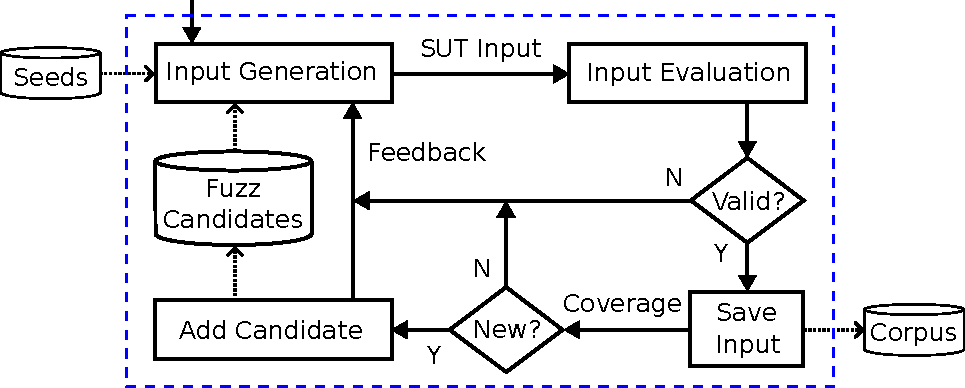
\includegraphics[width=0.9\linewidth]{figures/chapter5/Coverage-Guided Fuzzing.pdf}
    \caption{Coverage-Guided Fuzzing}
    \label{fig:fuzzing}
\end{figure}

The overall workflow of a fuzzing technique is given in Figure~\ref{fig:fuzzing}.
% 
The system under test is first tested with some set of random test inputs or a test suite that is manually generated.
% 
The outcomes of these test inputs, for example, coverage metrics like code coverage, or branch coverage are then evaluated and stored as test outputs.
% 
The coverage driven fuzzer assesses the various outputs of the inputs and selects a specific subset of tests to be added to seed collection.
% 
The fuzzer then assigns potential function to each of the seeds and generates a new test input by applying one of the mutator functions that can be either specified by the user or standard mutators that are available in the library.


In the case of AVs navigating through intersections, we automatically generate the behavior of all the non-ego vehicles.
% 
This includes generating the velocity profiles, the entry and exit lanes, and the turn indicators of all the vehicles.
% 
Based on the formalization of traffic rules, we then collect all the predicates that are triggered by the behavior of both the AV and the non-ego vehicles.
% 
Given a specific test scenario, the fuzzer asssess the importance of a given test input based on the new collection of predicates that are triggered by it.
% 
The mutators that change the given test scenario change 1) the entry and exit lanes of non-ego vehicles, 2) the velocity profile of the vehicles, and 3) the various turn signals associated with each behavior.
% 

